\documentclass[twocolumn]{article}
\usepackage[utf8]{inputenc}
\usepackage[T1]{fontenc}
\usepackage[english]{babel}
\usepackage{ifpdf,amsmath,amsthm,amssymb,amsfonts,newtxtext,newtxmath} 
\usepackage{array,graphicx,dcolumn,multirow,hevea,abstract,hanging}
\usepackage[labelfont=sc,textfont=sf]{caption}
\usepackage[hyperfootnotes=false,breaklinks=true]{hyperref} % was dvipdfmx
\urlstyle{rm}
%\usepackage[hyphenbreaks]{breakurl}
\usepackage{apacite} % must come afer hyperfootnotes
\setlength{\bibleftmargin}{1em}
\setlength{\bibindent}{-1em}
\usepackage{booktabs} % \toprule \midrule \bottomrule \cmidrule(lr){a-b}

%%%% Added by Zhenbo Cheng
\usepackage{subcaption}
%%%%%%%%%%%%%%%%%%%%%%%%

% define centered and ragged columns:
\newcolumntype{L}[1]{>{\raggedright\arraybackslash }p{#1}} % can use m{}
\newcolumntype{C}[1]{>{\centering\arraybackslash }p{#1}}
\newcolumntype{R}[1]{>{\raggedleft\arraybackslash }p{#1}}
\newcolumntype{d}[1]{D{.}{.}{#1}} % d{3.2} for 3 places on l, 2 on r
\newcommand{\mc}{\multicolumn}
\topmargin=-.3in \oddsidemargin=-.1in \evensidemargin=-.1in \textheight=9in \textwidth=6.8in
\setlength\tabcolsep{1mm}
\setlength\columnsep{5mm}
\setlength\abovecaptionskip{.5ex}
\setlength\belowcaptionskip{.5ex}
\setlength\belowbottomsep{.3ex}
\setlength\lightrulewidth{.04em}
\renewcommand\arraystretch{1.2}
\renewcommand{\topfraction}{1}
\renewcommand{\textfraction}{0}
\renewcommand{\floatpagefraction}{.9}
% \renewcommand{\baselinestretch}{1.00} \large\normalsize % for fixing spaces
\widowpenalty=1000
\clubpenalty=1000
\setlength{\parskip}{0ex}
\let\tempone\itemize
\let\temptwo\enditemize
\let\tempthree\enumerate
\let\tempfour\endenumerate
\renewenvironment{itemize}{\tempone\setlength{\itemsep}{0pt}}{\temptwo}
\renewenvironment{enumerate}{\tempthree\setlength{\itemsep}{0pt}}{\tempfour}

%%%%%%%%%%%%%%%%%%%%%%%%%%%%%%%%%%%%%%%%%%%%%%%%%%%%%%%%%%%%%%%%%%%%%
\setcounter{page}{1} % start with first page

\title{Strategies using recent feedback lead to matching or maximising behaviours}

\author{
Zhenbo Cheng\thanks{Department of Computer Science and Technology, Zhejiang University of Technology, Hangzhou, China}\;\,
\and 
  Jingying Gao\footnotemark[1]
\and
  Leilei Zhang\footnotemark[1]
\and
  Gang Xiao\footnotemark[1]\thanks{Email: xg@zjut.edu.cn}\;\,
\and
  Hongjing Mao\thanks{Mental Health Center Zhejiang University School of Medicine, Hangzhou, China } \thanks{Email:maohj1108@163.com}
}

% who is corresponding author?

\date{} % leave empty
\begin{document} % goes here

% fill in short title
\newcommand{\jref}{http://journal.sjdm.org/vol13.2.html}
\newcommand{\jhead}{Judgment and Decision Making, Vol.~13, No.~2}
\newcommand{\jdate}{March 2018}
\pagestyle{myheadings} \markright{\protect\small \href{\jref}{\jhead}, \jdate \hfill Strategies of matcching and maxmizing \qquad}
\begin{htmlonly}
\href{\jref}{\jhead}, \jdate, pp.\
\end{htmlonly}
%\begin{latexonly}
\twocolumn[
\vspace{-.3in}
{\small \href{\jref}{\jhead}, \jdate, pp.\ XX--XX}
%\end{latexonly}

\maketitle

%\begin{latexonly}
\vspace{-3mm}
\begin{onecolabstract}
%\end{latexonly}
  One challenge facing humans (and nonhuman animal) is that some
  options that appear attractive locally may not turn out best in the
  long run. To analyse this human learning problem, we explore human
  performance in a dynamic decision-making task that places local and
  global rewards in conflict. We found that experiences that included
  previous choices and rewards are not easily incorporated into
  people’s strategy to enhance their performance. Our results suggest
  that humans are easily driven by concerns about recent feedback, and
  that choice of a suboptimal behaviour option may be overcome by
  providing informative cues that indicate a clear immediate outcome
  for a better option.

\smallskip
\noindent
Keywords: matching law, optimal strategy, melioration strategy
%\begin{latexonly}
\end{onecolabstract}\bigskip
]
%\end{latexonly}

{\renewcommand{\thefootnote}{}
\footnotetext{ % note blank lines above and below acknowledgment

  This work is supported by Public Projects of Zhejiang Province
  (2016C31G2020069) and the 3rd Level in Zhejiang Province “151
  talents project” to Zhenbo Cheng. We thank Liwen Bianji, Edanz Group
  China (www.liwenbianji.cn/ac), for editing the English text of a
  draft of this manuscript. The authors declare no competing financial
  or nonfinancial interests.

Copyright: \copyright\ 2018.
The authors license this article under the terms of the
\href{http://creativecommons.org/licenses/by/3.0/}{Creative Commons
  Attribution 3.0 License.}
}}

\saythanks

\setlength{\baselineskip}{12pt plus.2pt}

\section{Introduction}

People often need to make rapid decisions on the relative allocation
of behaviour between competing alternatives in daily life. The choice
for each alternative may lead to a conflict with immediate and
long-term consequences. For instance, after a day in class, a student
may face a choice between exercising versus playing computer
games. Students might harm their long-term health by choosing to play
a computer game for long periods rather than to exercise because
playing a game gives an immediate reward and is therefore more
attractive. There is a famous experiment known as the Harvard Game
that examines how humans navigate decisions with conflict in the
immediate and long-term consequences \cite{RN1}.

In the Harvard Game, participants were asked to make an uninterrupted
sequence of choices between two alternatives (matching and maximising
options) with the goal of maximising the rewards they receive over the
entire session. On a given trial, the matching (suboptimal) option
always returns more reward than the maximising option. However, the
more the matching option is chosen, the less the future utility of
both alternatives becomes. Therefore, to receive maximal total rewards
in the game, participants on every trial need to choose the maximising
option that appears, at the time, to be the inferior option of the
two.

Over the past several decades, numerous behavioural results in the
Harvard game or variations of the game \cite{RN4,RN3,RN5,RN20} have
shown that humans and other animals often fail to inhibit the tendency
to select the matching option with higher local rates of reward, a
phenomena referred to as melioration \cite{RN6,RN7}. Melioration
deviates from rational choice in the consideration of local rates of
reward (suboptimal or melioration strategy) rather than the global
maximisation of utility (optimal or maximising strategy). According to
the melioration theory \cite{RN6}, human (or other animal) choice is
governed by a myopic tendency towards alternatives with higher local
rates of reward. However, the melioration strategy does not explain
how the optimal behavioural result might emerge from tasks that have
a reward structure similar to the Harvard game.

The present study was to examine how people could discover the optimal
strategy in such Harvard-type games through the use of additional cues
to indicate the increment of reward over rounds for each option. The
experimental paradigm that we used are rising optimum tasks
\cite{RN10,RN11,RN2}, which are an extension of the Harvard Game. In
experimental condition 1, we largely established that behaviour in the
task replicates previous work. In experimental condition 2, we
presented an extension of the task by providing participants with past
actions and rewards indicative of the underlying reward
contingencies. We find that a snapshot of recent experiences by itself
\cite{RN2,RN8,RN14,RN17,RN23,RN24,RN25} is insufficient to facilitate
participants acquiring optimal strategy. In experimental condition 3,
we rearranged past choices and rewards, showing the sequence for each
alternative separately, to help participants to understand the change
of reward over rounds for each option. This display was effective in
helping participants learn to make the optimal choice.

\section{Method}

A total of 141 undergraduate students from Zhejiang University of
Technology participated in three conditions (69 males, 72 females;
ages ranging from 18 to 22, with a mean age of 19.8). All of them had
normal or corrected-to-normal vision and normal colour vision. They
were randomly divided into three groups, with 47 participants in each
of the three conditions. They were told that they would earn money
according to the total score they obtained in a sequential two-choice
task.

The experimental equipment was a Lenovo Shaoyang desktop computer, the
display equipment was a 17-inch flat CRT monitor, the screen
resolution was set to 1024 $\times$ 768 pixels, and the mouse
resolution was 1000 dpi.

The three different conditions are shown in the Figure 1A--C. In each
condition, participants choose sequentially between two actions by
pressing one of the two buttons: A or B. Clicking on the button A or B
cause the colour bar (red or cyan, respectively) in a square window to
update, and the height of the bar indicated the score from that
choice. The cumulative score of the choices is displayed numerically
in the upper part of the rectangle window. In the second condition,
the recent choices (at most 20 trials) before the current trial are
displayed on the top of the screen (Figure 1B). In the third
condition, the recent choice is displayed beside the two buttons,
respectively. After each choice, the little bar is separately
displayed beside the two buttons according to the choice. As shown in
Figure 1C, the button A is chosen in the first trial, and then the B,
A, A, A and B buttons are selected in turn in next five trials. After
the sixth trials, the four (two) red (cyan) little bars are displayed
beside the button A (B).

\begin{figure}[t!]
%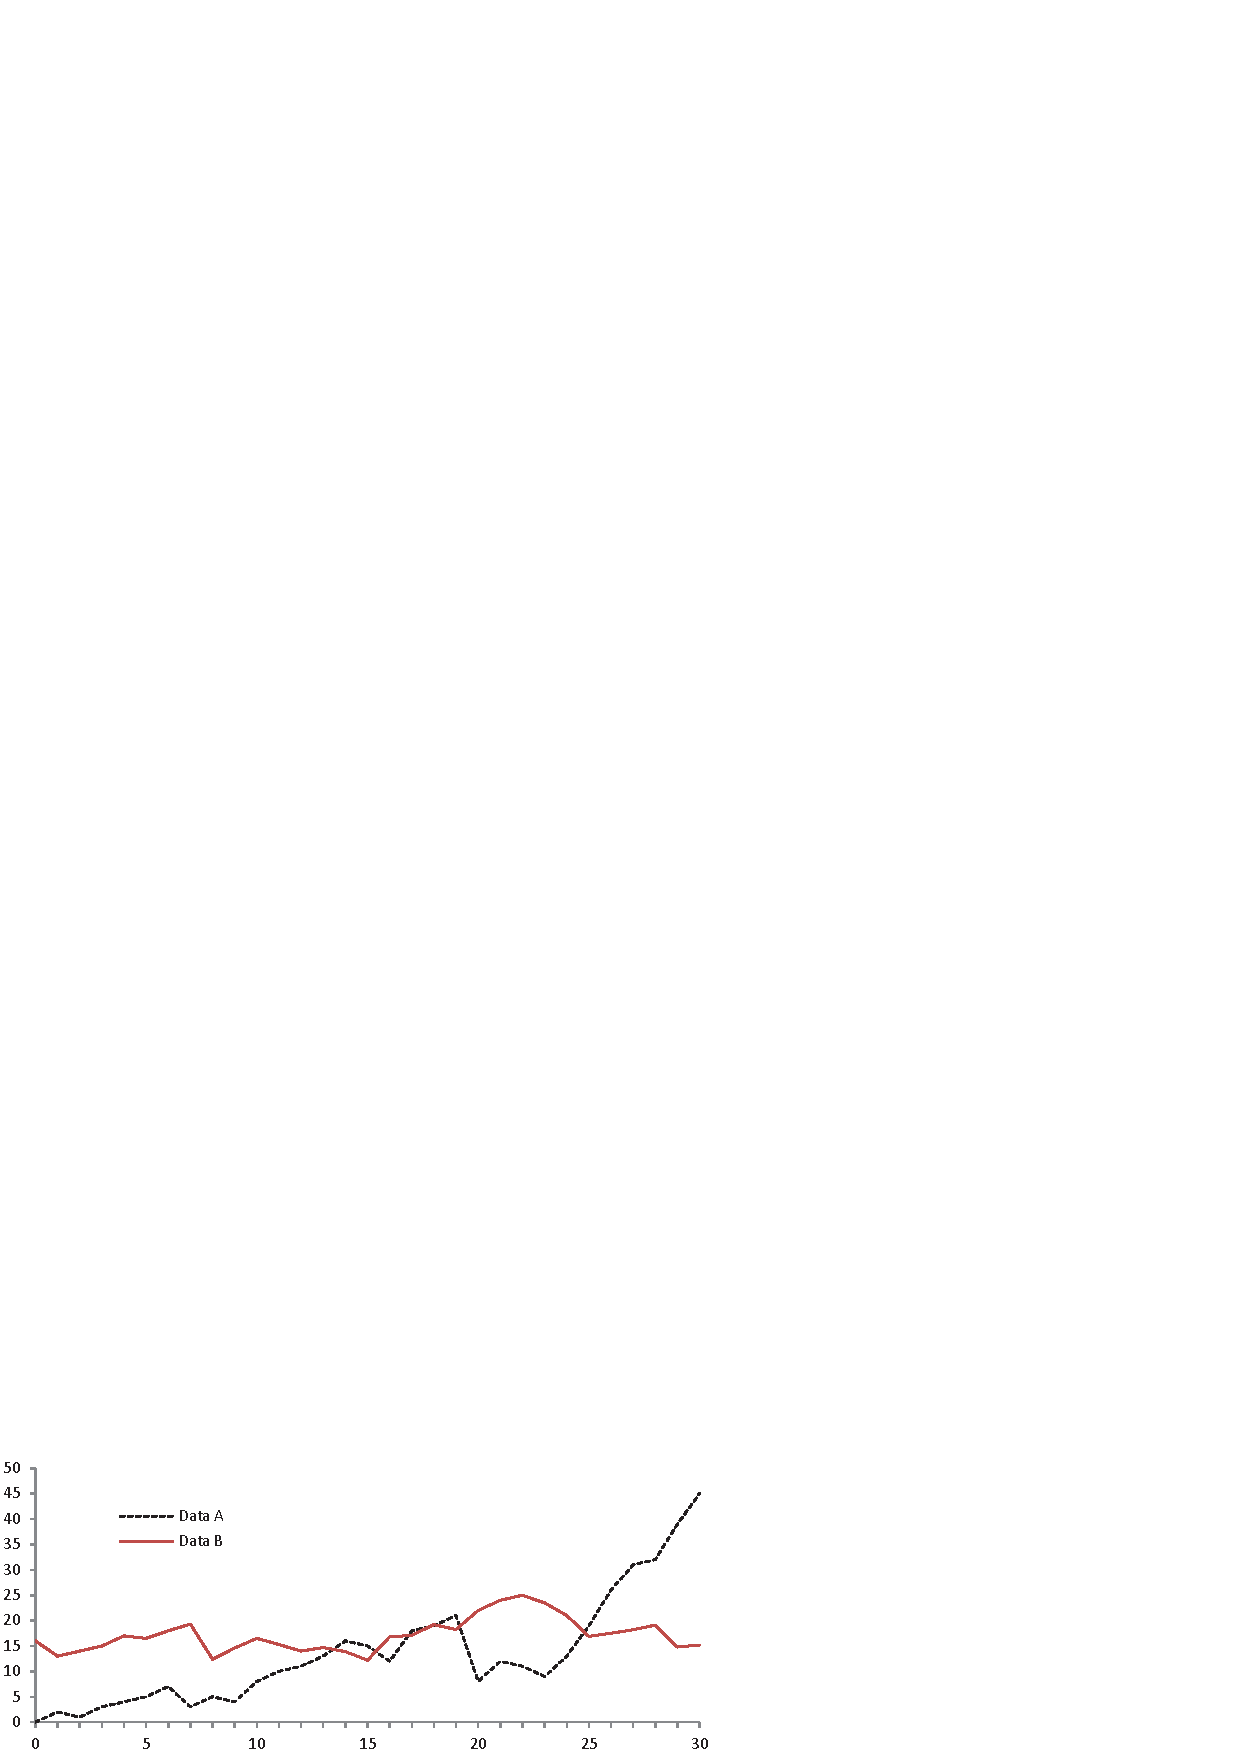
\includegraphics[width=\columnwidth]{fig1.pdf}
\caption{The task and reward structure. A-C) the three conditions in
  the task. A) Sample two trials during the first condition. The
  participant selects the button A and obtain score of 55 in the first
  trial. Then the button B is chosen in the second trial and obtain
  score of 38. After each choice, a scale bar is updated to reflect
  the reward earned for that choice, and the bar height following a
  choice depends on the obtained score for that choice. B) The
  previous choices and scores are shown on the top of the screen in
  the second condition. C) The previous choices and scores are
  separated on both sides of the screen according to the choices in
  the third condition. D) Reward functions (blue and green curve) for
  two choices as the function of choice allocation to A. The dashed
  red curve shows the utility rate for different proportions of
  responses to A.}
\end{figure}

On each trial, the reward is a function of past choices. Such history
dependence is modelled through the reward equation used for the same
purpose by Montague and Berns (2002), as follows:
\begin{equation}
R_i(q)= 
\begin{cases}
g \times (c_1-c_2\sqrt{q_A(t)\times W}),& a_A(t)=1 \\
g \times (c_3-\frac{1}{1+\exp{(-c_4\times q_A(t)\times W})}),& a_B(t)=1
\end{cases}
\end{equation}
where $g$, $c_1$, $c_2$, $c_3$ and $c_4$ determine the shape of the
function $R$. $q_A(t)$ is the ratio of chosen button A over the last
$W$ (= 20) trials. The $q(t)$ is defined as
\begin{equation}
q_i(t)=\frac{\sum_{\tau=1}^{W}a_i(t-\tau)}{W}, i=A/B
\end{equation}
where $a_i(t)$ is participant’s choice at trial $t$. If the button A
is chosen, $a_A(t)$ = 1 and $a_B(t)$ = 0; if button B is chosen,
$a_A(t)$ = 0 and $a_B(t)$ = 1. We refer to the proportion of A choices
in the last $W$ trials as allocation to A.

As shown in Figure 1D, the blue curve shows the score after pressing
button A for different allocations to A during the last 20 trials, and
the green curve shows the score after pressing button B
($g = 240, c_1 = 1.05, c_2 = 0.215, c_3 = 1.2$ and $c_4 = 0.4$). For
example, if the participant had pressed equal number of A and B within
the last 20 trials and the last choice was A, then the resulting score
is 92 --- it can be read from Figure 1D by looking at blue line.

The matching behaviour is at the intersection of the blue and green
lines in a way that the returns of the two alternative targets are
equal \cite{RN26,RN27}. Thus, the strategy for matching behaviour is
to choose button A (matching target) with probability 0.75. The
crossing point of the blue and green lines is called the matching
point. The dashed red line in Figure 1D is the utility rate for
different proportions of responses to A. The utility rate is defined
as the global average rate of return from the two alternatives. To
gain the maximal reward, participants need to press button B
(maximizing target) on every choice. Thus, the far left end point of
the red dashed curve is called the optimizing point. For simplicity,
we call the matching target button A, and the maximizing target button
B. In fact, button A and button B were randomly assigned to the
matching target and the maximising target for each participant.

Participants were instructed to maximise the reward (score) over the
course of the task. Each participant had 10 trials to familiarise
themselves and performed 100 trials during each condition. The cash
they gained is equal to the total score ($\times$ 0.001 CNY) after
conducted a condition.

\section{Results}

Figure 2 shows the average proportion of matching alternative and
average reward rate for each participant in the three conditions,
where each black point represents a participant. In conditions 1 and
2, except for a few outliers, all participants chose on average to
stay near the matching point rather than the optimising point. In
condition 3, however, a majority of participants chose on average to
stay near the optimising point.

\begin{figure}[t!]
%\includegraphics[width=\columnwidth]{fig2.pdf}
\caption{Average proportion choice A and average reward rate for each participant (black points), overlaid over the reward structure for button A (blue) and B (green).}
\end{figure}

Figure 3 shows the distribution of choice A and reward. Most
participants chose to stay with the point in which the allocation to A
was near 0.7 in conditions 1 and 2. At this point, the total score
(reward) roughly equals to 5000. In condition 3, some participants
chose to stay at the point where the allocation to A was near 0. At
this point, the total score was approximately 12,000. The difference
in total score between conditions 2 and 3 was significant at $p<.001$
by a t test.

\begin{figure}
    \centering
    \begin{subfigure}[b]{0.45\textwidth}
        %\includegraphics[width=\textwidth]{fig3_1}
    \end{subfigure}
    ~ 
    \begin{subfigure}[b]{0.45\textwidth}
        %\includegraphics[width=\textwidth]{fig3_2}
    \end{subfigure}
 
    \caption{Distributions of allocation to A (top panels) and total rewards (bottom panels) in the three conditions.}
\end{figure}

To more precisely quantify participants' behaviour with regard to type
of strategy, we calculated the fraction of trials that followed the
optimal and the melioration strategies for each participant. Because
the optimal strategy is always to choose option B, we define the
optimising fraction simply as the fraction of choices B. In addition,
the meliorating fraction is defined as the proportion of choices that
satisfy this strategy among the trials where the allocation to A was
between 0.72 and 0.82. For each subject, we determined the strategy
that was followed on the greatest number of trials. The fraction of
all participants with a preference of each strategy in two conditions
is shown in Figure 4. In conditions 1 and 2, nearly 60\% of
participants adopted the melioration strategy, whereas, in condition
3, only about 25\% of participants adopted the melioration strategy,
and about 55\% of participants adopted the optimal
strategy. Interestingly, not all of behavioural results of
participants reached the matching or maximising points.

\begin{figure}[t!]
%\includegraphics[width=\columnwidth]{fig4.pdf}
\caption{Proportion of participants with melioration and optimal strategy in the three conditions.}
\end{figure}

\section{Discussion}

We used rising optimum tasks, which have been used previously to
investigate simple reinforcement learning behaviour and short-term
memory traces for action bias in human sequential decision-making
\cite{RN2}. We examined the effects of recent experiences on choice in
the rising optimum task that placed short- and long-term rewards in
conflict. The results of our first condition showed that most
participants become stuck in a local cycle around the matching point
of the reward curves where the fractional allocation to target A is
approximately 0.75, which are consistent with several previous studies
\cite{RN2,RN12}. Furthermore, the results of the second condition
demonstrated the snapshot of recent experiences is insufficient to
facilitate participants acquiring optimal performance in the task,
where the fractional allocation to target B is nearly 1. In the third
condition, we found that participants more easily reach optimal
performance by adding cues to indicate the increment of reward for
each option, separately, so that the change over rounds was more
salient.

Participants in the first condition appear to have favoured the
matching option, although they can obtain the maximal total income by
selecting the maximal option on every choice. However, the optimal
strategy is not obvious to the participants because choosing A results
in greater immediate reward than choosing B for allocations A lesser
than 0.7. Continuing to select A will produce gradually lesser reward
(diminishing return), but these will remain greater than selecting B
until the allocation to A higher than 0.7. At that point, choosing B
will obtain greater immediate reward than choosing A. Thus, most of
participants in the first condition reach matching behaviour since
they are driven primarily by concerns about immediate reward.

Participants could adopt the optimal strategy while they learn to take
account of the recent history of actions. However, most of the
participants kept adopting the melioration strategy even though the
snapshot of recent experiences is given in the second condition.  The
existing theory often uses the eligibility trace model of
reinforcement learning to explain the decision-making results
converging to the optimisation point in the rising optimum task
\cite{RN2,RN16}, but the eligibility trace model requires the
participants to take advantage of all of the past experience. The
behavioural results in condition 2 demonstrated that even given the
necessary information (i.e., the snapshot of recent experiences) for
the optimal strategy, the participants still find it hard to find the
strategy \cite{RN21,RN22,RN15}.

In the third condition, we rearranged past choices and rewards for
each alternative to help participants to easily find payoffs from
consecutively choosing the target A decrease, whereas the payoff from
consecutively choosing the target B increase. Thus, participants in
the third condition could directly perceive the increment of payoff on
each option. The behavioural results in condition 3 indicated that
providing cues indicating the immediate feedback about the increment
of payoff to participants could make it easier for participants to
adopt the optimal strategy. Our finding in the third condition is
largely consistent with previous works demonstrating how cues
indicative of underlying dynamics for decision-making task may help
decision makers develop optimal strategies \cite{RN12,RN13,RN28}. For
example, perceptual cues that readily align with the underlying state
of the Farming on Mars task environment help participants overcome the
impulsive appeal of short-term rewards \cite{RN12}. The participants
were more likely to maximise profit when provided with an arrow that
indicated the number of responses the participant made to the
maximising choice option over the relevant choice history
\cite{RN13}. Our results indicate that preferring the option for local
payoff can, in some circumstances, be overcome by providing
informative cues that indicate a clear immediate outcome for another
option.

\bibliographystyle{apacite}
\bibliography{mybib.bib}



\bigskip


\end{document}

